\chapter*{Введение}                         % Заголовок
\addcontentsline{toc}{chapter}{Введение}    % Добавляем его в оглавление

Гидроразрыв пласта (ГРП) — один из эффективных методов интенсификации нефтеотдачи. Суть данного метода заключается в следующем. При помощи закачки вязкой жидкости на забое скважины создается избыточное давление, достаточное чтобы преодолеть минимальные горные напряжения и разорвать горную породу. Порода разрывается вдоль поверхностей минимальных напряжений в пласте, и за счет гидродинамического воздействия жидкости в породе начинает расти и раскрываться трещина. Ввиду сложности физических процессов и недоступности прямому наблюдению развития трещины гидроразрыва пласта, для оценки технологических параметров при проведении ГРП и геометрических размеров созданной трещины применяют специализированное программное обеспечение — симуляторы гидроразрыва пласта.

Для математического моделирования ГРП целевой пласт представляется в виде слоистой среды, где каждый слой считается упругим изотропным сплошным телом, обладающим своими модулями упругости. Помимо точности численных методов для моделирования ГРП не менее важна скорость расчётов. Симуляторы ГРП, основанные на методе конечных элементов (МКЭ), применимы для задач с неоднородной средой, однако требует большие вычислительные затраты. Поэтому возникает потребность в менее ресурсоёмких методах.

\begin{figure}[htbp]
    \centering
    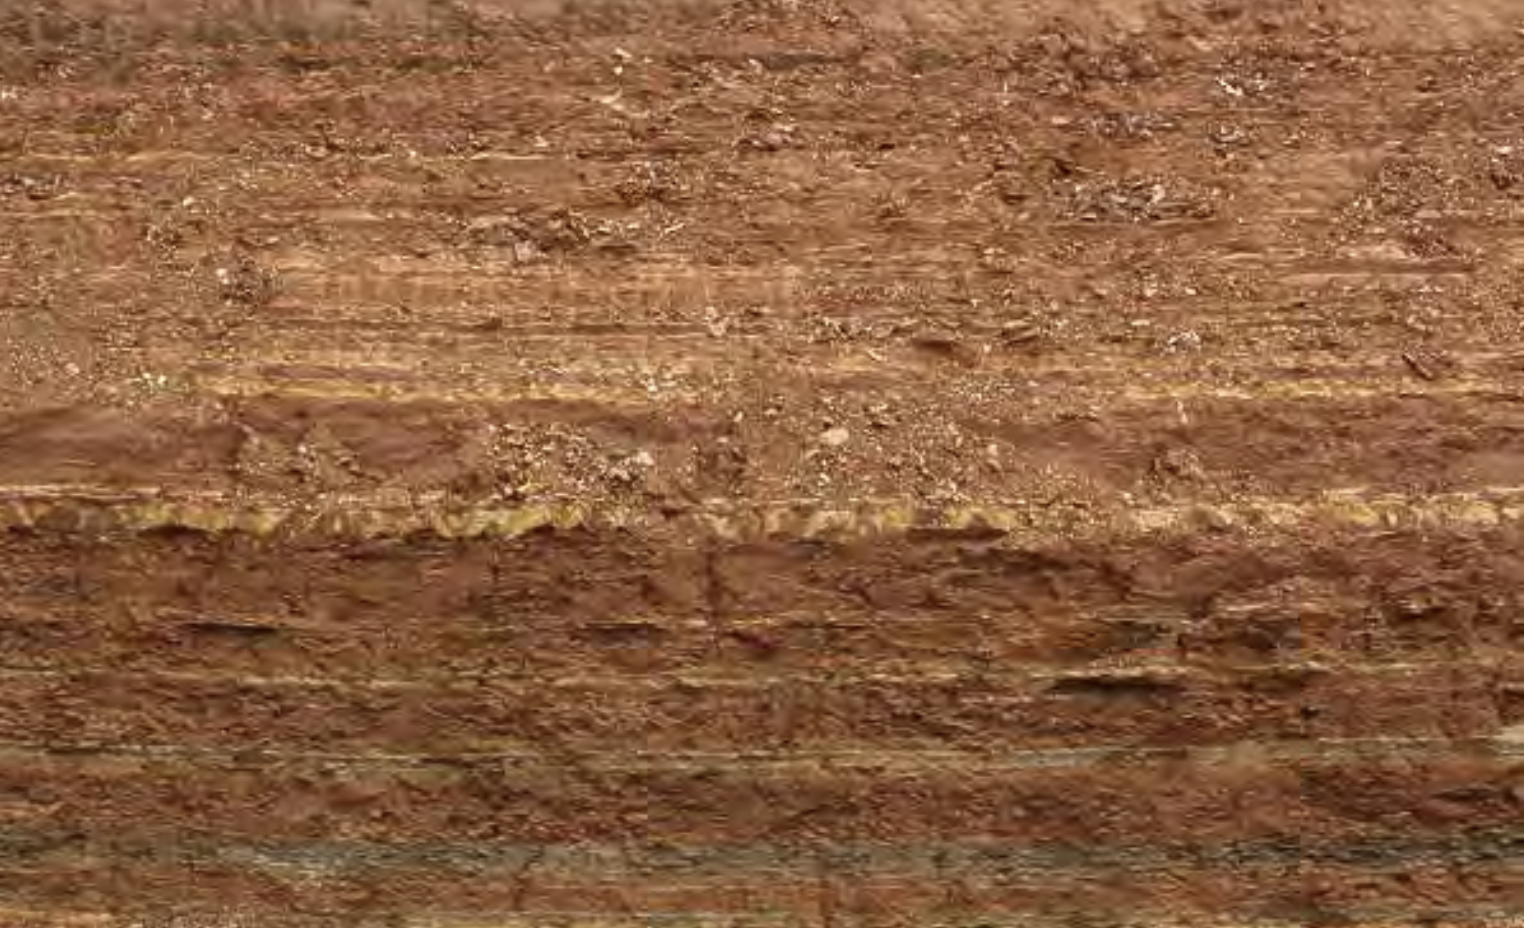
\includegraphics[width=0.8\textwidth]{layered-structure.png}
    \caption{Слоистая структура горной породы.}
\end{figure}

Модель Planar3d ILSA \cite{DONTSOV201753}, используется для моделирования плоских трещин. Она основана на методе разрывных смещений (МРС), \cite{dispalecement_discontinuty_Crouch1983}), в котором расчетная сетка строится только на границе области, что позволяет уменьшить размерность матрицы упругости на единицу за счет использования аналитического решения для однородной изотропной среды \cite{Peir2008}. Для слоистой среды не существует аналитического выражения для коэффициентов матрицы упругости, поэтому для обобщения данной модели использует следующие подходы.

Первый заключается в гомогенезации (осреднение) модулей упругости по всем слоям \cite{DONTSOV2021108144}. Преимуществом данного подхода является относительно простая реализация, за счет введения средних модулей упругости и сведения задачи к однородной изотропной среде. Однако данный подход не применим для слоистых структур с большой разницей упругих модулей и сред с включением тонких жестких пропластков.

Второй подход основан на численном построение матрицы упругости \cite{Siebrits_Peirce_2002,Peirce2001TheSF,Peirce2001UniformAA,Linkov1992}. Для этого применяют двумерное преобразование Фурье для определяющих уравнений упругой среды и далее, учитывая условия непрерывности компонент вектора смещений и нормальной нагрузки на границе раздела слоев, решают связанную задачу. После этого матрицу упругости можно восстановить путем применения обратного дискретного преобразования Фурье к полученному решению.

Целью данной работы является реализация метода построения численной матрицы упругости для слоистой среды с неоднородностью по модулям упругости и внедрение его в модель Planar3d ILSA. В работе показано существенное влияние неоднородности модулей упругости на геометрию трещины ГРП. Приведены примеры, связывающие неоднородность сжимающих горных напряжений с неоднородностью модулей упругости в пласте. Рассмотрены слоистые структуры, включающие тонкие жесткие пропластки.


\clearpage